%--- Heterogeneity by exposure to the 2010 Maule earthquake (MMI > 7), all adopters
\begin{figure}[h!]
    \centering
    \caption{Effects of \emph{Plan Cuadrante} by Exposure to the 2010 Earthquake}
    \label{fig:heterogeneity_earthquake_mmi}
    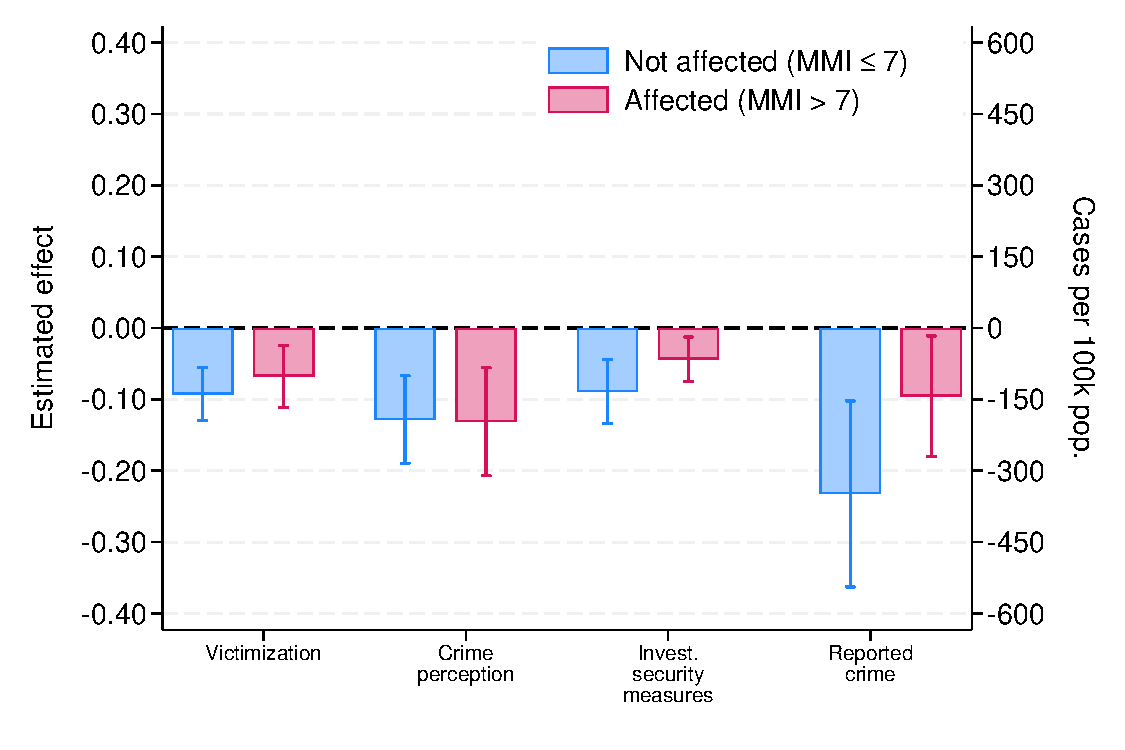
\includegraphics[width=0.8\textwidth]{../manuscript/Graphs/heterogeneity_earthquake_mmi.pdf}
    \\[10pt]
    \begin{minipage}{0.99\textwidth}
    \footnotesize
    Notes: This figure reports the heterogeneous effects of \emph{Plan Cuadrante} by exposure to the 2010 Maule earthquake, estimated separately for municipalities more exposed to the earthquake---defined as those with a Modified Mercalli Intensity (MMI) greater than 7, ``affected'' (red bars)---and municipalities with an MMI of 7 or lower (``not affected'', blue bars), using all adopters. For each exposure group, we estimate the pooled post-treatment effect of the program with the difference-in-differences estimator for staggered adoption of \citet{Callaway}, comparing municipalities of the same exposure level to each other so that the earthquake's direct effect on outcomes is differenced out within each group. Victimization is the probability of household victimization in the last 12 months; crime perception is the probability of perceiving an increase in crime; and investment in security measures is the probability of adopting security measures in the last twelve months---all from the ENUSC survey and read on the left axis. Reported crime is the number of crimes reported to the police per 100,000 inhabitants, from administrative data, and read on the right axis. Bars represent the average post-treatment effect and the whiskers the 95\% confidence intervals; standard errors are clustered at the municipality level using the wild bootstrapping procedure.
    \end{minipage}
\end{figure}
